\documentclass{report}

\usepackage{amsmath, mathrsfs, amsthm}
\usepackage{graphicx}
\usepackage{etoolbox}
\makeatletter
\patchcmd{\chapter}{\if@openright\cleardoublepage\else\clearpage\fi}{}{}{}
\makeatother

\title{Ragionamento Automatico: Tree Decomposition}
\author{Brian Riccardi}
\date{}

\newtheorem{defi}{Definizione.}
\newtheorem{prop}{Proposizione.}
\newtheorem{lem}{Lemma.}
\newtheorem{teo}{Teorema.}
%\newtheorem{proof}{Dim.}

\begin{document}
\maketitle
\tableofcontents

\newpage

\chapter{Il problema}
Il problema che vogliamo risolvere è la ricerca di una \textit{tree decomposition} di \textit{width} minima di un grafo non orientato G.
Verranno utilizzate le tecniche di programmazione con vincoli (Minizinc) e di programmazione di tipo Answer Set (ASP/clingo).

\section{Definizioni e osservazioni}

Procediamo dando una definizione formale del problema e una serie di definizioni che utilizzeremo in seguito.

\begin{defi}(\textbf{Tree Decomposition})\\
Sia $G = (V_G, E_G)$ un grafo non orientato, $T = (V_T, E_T)$ un albero e \\$\chi{}: V_T~\longrightarrow{} \mathscr{P}(V_G)$.
Diremo che $\tau = (T, \chi)$ è una \textit{tree decomposition} per $G$ se e solo se:
\begin{description}
	\item[TD1:] $\displaystyle\bigcup_{t \in V_T}{\chi{}(t)} = V_G$
	\item[TD2:] Per ogni arco $uv \in E_G$ esiste $t \in V_T$ tale che $\{u, v\} \subseteq \chi{}(t)$
	\item[TD3:] Per ogni terna $r, s, t \in V_T$ tale che $s$ si trovi nel cammino da $r$ a $t$, vale $\chi(r) \cap \chi(t) \subseteq \chi(s)$
\end{description}
\end{defi}

\begin{defi}(\textbf{Width})\\
Data una \textit{tree decomposition} $\tau = (T, \chi)$, definiamo \textbf{treewidth} la quantità \\
$w(\tau) = \displaystyle\max_{t \in V_T}\{|\chi{}(t)|\}-1$.
\end{defi}

\begin{defi}(\textbf{Minimal tree decomposition})\\
Dato un grafo $G$ non orientato, il problema della \textit{minimal tree decomposition} è la ricerca di una tree decomposition per $G$
di \textit{width} minima. Se tale decomposition ha width $w(\tau)=k$, allora diremo che $G$ ha treewidth $w(G)=k$.
\end{defi}

Da questo punto in poi daremo per scontato che ogniqualvolta si parli di una tree decomposition, questa sia riferita a un grafo $G$ non orientato di $n$ nodi
e che la decomposition sia $\tau = (T, \chi)$.

Il concetto di tree decomposition può essere visto come una variante del problema della colorazione: possiamo infatti immaginare i nodi dell'albero
come a dei colori e la funzione $\chi$ come a un'assegnamento dei colori ai nodi. In particolare, per (\textbf{TD3}) viene richiesto che ogni nodo del grafo
venga colorato con un sottoalbero di $T$ e per (\textbf{TD2}) viene richiesto che i rispettivi sottoalberi si intersechino. Dato questo cambio di prospettiva spesso
parleremo di \textit{colori} quando ci riferiremo ai nodi di $T$.

La prima osservazione che uno può fare è che non esiste una decomposition unica; inoltre, non è immediato dare un limite superiore a $|V_T|$ tale che
$T$ induca una decomposition minimale. In particolare, tale bound è utile ai nostri scopi: ci permette di definire dei modelli (a vincoli o answer set) più efficaci.
\ \\

Diamo ancora qualche definizione che ci sarà utile nella prossima sezione.
\begin{defi}
Dato un albero $T = (V, E)$ e un arco $uv \in E$, definiamo la \textbf{contrazione} di $uv$ come l'albero $T/uv$ dove i nodi $u, v$ vengono rimpiazzati da un nodo
$\overline{uv}$ e gli archi incidenti a $u$ e $v$ diversi da $uv$ diventano ora incidenti a $\overline{uv}$.
Data una tree decomposition $\tau$ e un arco $uv \in E_T$, la contrazione di $uv$ induce $\chi_{uv}: V_{T/uv} \longrightarrow \mathscr{P}(V_G)$ definita da
\begin{align*}
\chi_{uv}(t) = \begin{cases}
										\chi(t) 							 & \text{ se } t \neq \overline{uv}\\
										\chi(u) \cup \chi(v)  & \text{ se } t = \overline{uv}
							  \end{cases}
\end{align*}
Diremo che $uv$ è $\tau$\textit{-contraibile} se e solo se la coppia $(T/uv, \chi_{uv})$ è una decomposition\footnote{Non è difficile verificare che le decomposition
sono chiuse per contrazione.} di treewidth \textbf{non maggiore}.\\
Diremo inoltre che $\tau$ è contraibile se ammette un arco $\tau$-contraibile, \textbf{completamente contratto} altrimenti.
\end{defi}

\section{Lemmi e teoremi}
In questa sezione ci preoccuperemo di derivare la bound menzionata precedentemente; vedremo infatti che un qualsiasi grafo di $n$ nodi ammette
una tree decomposition minimale di al più $n$ colori.

\begin{lem}\ \\
Siano $r, s$ colori tali che $\chi(r) \subseteq \chi(s)$. Allora $rs$ è $\tau$-contraibile.
\end{lem}

\begin{proof} Banale.
\end{proof}
 

\begin{lem}
Sia $\tau$ una decomposition di $m > n$ colori, allora esistono $r, s$ tali che $\chi(r) \subseteq \chi(s)$.
\end{lem}

\begin{proof}
Supponiamo per assurdo che tali colori non esistano e fissiamo una foglia $l$ di $T$ e il suo vicino $h$. Per ipotesi, esiste $x \in \chi(l)$ tale che $x \notin \chi(h)$.
Consideriamo dunque una visita in profondità dell'albero a partire da $l$ con lo scopo di enumerare i nodi di $G$. Tale enumerazione sarà la successione $\{\sigma_i\}_{i \in 1\dots{}m}$

In particolare:
\begin{itemize}
	\item $\sigma_1 := x$
	\item Al passo $k>1$ della visita, quando entro in un nuovo colore $s$ arrivando da $r$, $\sigma_k := y$ tale che
						$$\begin{cases}y \in \chi(s),\\ y \notin \chi(r), \\ \forall{i<k}( y \neq \sigma_i ) \end{cases}$$
\end{itemize}
L'esistenza di un tale $y$ è assicurata dall'ipotesi iniziale e da (\textbf{TD3}): se non esistesse un tale $y$, si avrebbe $\chi(r) \supseteq \chi(s)$ oppure
si avrebbe $\sigma_j=y$ per qualche $j<k-1$, ma allora verrebbe meno (\textbf{TD3}) in quanto $y$ avrebbe due colori distinti ma non ogni colore ``intermedio" (ovvero $r$, per costruzione).

Abbiamo quindi costruito una sequenza $\{\sigma_1, \sigma_2, \dots, \sigma_m\}$ di nodi distinti di $G$, ma questo è un assurdo in quanto per il Principio della Piccionaia ~---~essendo $m>n$~---~
almeno un nodo compare due volte in tale successione.

\end{proof}

I due lemmi, ci assicurano che qualunque sia una decomposition, se questa ha un numero sufficiente di colori allora sarà contraibile.

\begin{teo}(\textbf{Bounded decomposition})\\
Sia $G$ un grafo di treewidth $w(G)=k$, allora esiste una tree decomposition per $G$ di al più $n$ colori.
\end{teo}
\begin{proof}
Sia $\tau$ una tree decomposition minimale per $G$ con $m > n$ colori. Dai lemmi precedenti sappiamo che $\tau$ è contraibile e dunque,
applicando $m-n$ contrazioni sugli archi che soddisfano l'ipotesi del lemma 1, otteniamo una nuova tree decomposition minimale $\tau'$ di $n$ colori.
\end{proof}

\section{Idea risolutiva}

Il teorema della sezione precedente ci assicura che se ci concentriamo su decompositions di al più $n$ colori non rischiamo di perderci la soluzione ottima.
I modelli delle sezioni successive, quindi, si baseranno su questa idea.\\

Analizzando la definizione di decomposition balza subito all'occhio (\textbf{TD3}) che richiede una trattazione non banale: data una terna di colori, saper decidere
se un colore appartiene al path tra gli altri due.\\

Sebbene i due modelli utilizzino paradigmi differenti, l'idea alla base per la decisione di (\textbf{TD3}) si basa sul
concetto di \textit{Lowest Common Ancestor}\footnote{Ricordiamo che, in un albero radicato, il Lowest Common Ancestor tra due nodi $x, y$ è (l'unico) nodo $z = LCA(x, y)$ tale che
$x, y$ sono discendenti di $z$ e $z$ è massimale (rispetto alla profondità) tra i nodi che godono di questa proprietà.}; infatti, supponendo di aver radicato l'albero: siano $r, s, t$ i colori,
e $\mathcal{A}$ la relazione \textit{antenato di}, allora
$$s \in \pi_{rt}\;\; \longleftrightarrow\;\; s = LCA(r, t) \lor \big(s\mathcal{A}r \oplus s\mathcal{A}t\big)$$

Viene quindi naturale radicare l'albero e, per eliminare qualche simmetria:
\begin{itemize}
	\item Imporre sempre al nodo $1$ il ruolo di radice
	\item Enumare i colori dall'alto verso il basso imponendo parent$(x)<x$ e\\ $(x<y \longrightarrow depth(x) \leq depth(y))$
\end{itemize}

\chapter{Minizinc}

Minizinc è un linguaggio per \textbf{modellare} problemi esprimendoli come un insieme di domini, variabili e vincoli su queste variabili.

\section{Struttura del modello}

Nel modello sono presenti le costanti \texttt{N} e \texttt{graph} che rappresentano, rispettivamente, $n$ e la matrice di adiacenza di $G$. Si è poi
deciso di inserire una variabile intera \texttt{n} di dominio $[1, \texttt{N}]$ per rappresentare $|V_T|$. Sono presenti un insieme di variabili
\texttt{parent}, \texttt{depth} e \texttt{lca} di ovvia interpretazione, \texttt{ancestor} che decide se un colore è antenato di un altro (utile per vincolare
\texttt{lca}). Infine, sono presenti delle variabili binarie \texttt{hasColor} per decidere se un nodo ha un determinato colore.
\ \\
\ \\

La prima serie di constraints ha lo scopo di vincolare \texttt{parent} e \texttt{depth} per ottenere a tutti gli effetti un albero. Si preoccupano di applicare le idee
risolutive discusse precedentemente. In particolare, il predicato \texttt{non\_decreasing\_except\_0} è stato definito da me.
\ \\
\ \\

La seconda serie di constraints si occupa di vincolare la relazione di \texttt{ancestor} (che verrà utilizzata per il calcolo di \texttt{lca}). I constraints non sono complessi
da capire: ci preoccupiamo di vincolare a \texttt{0} tutto ciò che riguarda colori \textit{extra} (ovvero più grandi di \texttt{n}) e ci preoccupiamo di vincolare gli antenati
\textit{ovvi} (parent e figlio) ed esprimiamo una condizione necessaria e sufficiente (simil-induttiva) per vincolare un antenato al suo discendente. Viene poi impiegato un
vincolo ridondante per assicurarci che un colore con indice grande non possa essere considerato antenato di un colore con indice piccolo.
\ \\
\ \\

La terza serie di vincoli si preoccupa di costruire la tabella \texttt{lca}: dopo la solita \textit{pulizia} per rendere noto al solver che siamo interessati solo agli LCA di
colori $\leq$\texttt{n}, sono state inserite delle condizioni per assicurarci che \texttt{lca[x, y] <= min\{x, y\}}, delle condizioni per vincolare la simmetria
\texttt{lca[x, y]=lca[y, x]} e delle condizioni simil-induttive per il calcolo effettivo, nonché un vincolo per il calcolo di LCA quando un colore è antenato dell'altro.
\ \\
\ \\

Vengono poi espresse le tre condizioni di tree decomposition: ogni nodo ha un colore, due nodi adiacenti condividono un colore e se un nodo ha due colori distinti,
allora deve avere tutti i colori presenti nel percorso tra essi; per quest'ultimo, è stato definito un predicato \texttt{inPath}. Sono stati poi definiti dei vincoli per assicurarci
di usare ogni colore dell'albero e di non usare alcun colore al di fuori dell'albero. Viene espressa la variabile \texttt{objective} e vincolata ad essere la cardinalità massima
(meno 1) degli insiemi indotti dalla colorazione. Infine, vengono vincolati i colori affinché ogni $\chi(t)$ abbia cardinalità almeno la metà dell width nella speranza di aiutare
il solver a considerare meno casi (talvolta inutili): la correttezza del vincolo è data dal lemma sulle ``inclusioni".

\section{Search strategies}
Sono state provate diverse search strategies ma nessuna ha sortito grandi effetti sulla qualità della soluzione. Le strategie proposte in questa relazione riguardano
la scelta dei valori di \texttt{parent} e \texttt{depth}: in una viene applicata \texttt{int\_search(parent ++ depth, first\_fail, indomain\_min, complete)}, mentre
nell'altra \texttt{int\_search(parent ++ depth, first\_fail, indomain\_random, complete)}. Nel primo caso, si cerca di prediligere alberi il più possibile ``compatti", nel
secondo caso invece si cerca di non assumere alcuna euristica.

\chapter{ASP/clingo}

In un programma Answer Set vengono descritti un insieme di fatti e un insieme di regole di deduzione al fine di produrre un \textit{insieme stabile}.

\section{Struttura del modello}

Una relazione binaria \texttt{edge} descrive gli archi del grafo sottoforma di fatti (si è scelto di utilizzare solo uno dei due versi)., con una costante \texttt{n}
che rappresenta $n$ Sono presenti relazioni binarie \texttt{parent} e \texttt{hasDepth}, unarie \texttt{root} e \texttt{nt} per descrivere l'albero: in particolare,
\texttt{nt} determina il numero di nodi dell'albero. Vi sono relazioni binarie \texttt{hasColor} e \texttt{ancestor}, ternarie \texttt{lca} e \texttt{inPath} di ovvi significati.
\ \\
\ \\

Una serie di default permette di dedurre che ogni colore ha un'unica profondita (positiva nel caso in cui il colore non sia \texttt{root}) e questa profondità è strettamente
legata alla relazione \texttt{parent}; anche in questo caso si è deciso di eliminare qualche simmetria introducendo dei default che forzassero il modello ad assumere 
albero indicizzati dall'alto verso il basso.
\ \\
\ \\

Una seconda serie di default permette di descrivere le condizioni per una tree decomposition e per descrivere le relazioni
\texttt{lca} e \texttt{inPath}: entrambe vengono descritte facilmente, esprimendo simmetrie e definizioni induttive; in particolare, \texttt{inPath} sfrutta la solita proprietà
descritta precedentemente. Infine, viene definita una relazione binaria \texttt{size} per descrivere le cardinalità dei $\chi$, e una relazione unaria per descrivere
la funzione obbiettivo.

\section{Search strategies}
Sono stati effettuati due tipi di test: in uno è stato utilizzato \texttt{clingo} \textit{standard}, nell'altro è stata utilizzata l'opzione \texttt{--opt-strategy=bb}
che cerca di stabilire se una soluzione trovata è ottima ``dimostrando'' l'insoddisfacibilità di modelli di costo minore: questo approccio mi è sembrato interessante 
avendo a che fare con un problema dalle condizioni stringenti e dipendenti dalla struttura stessa del grafo (intuitivamente, più il grafo è denso e più la width è alta).

\chapter{Risultati sperimentali}

\begin{figure}
\centering

\begin{tabular}{ccc}[H]
	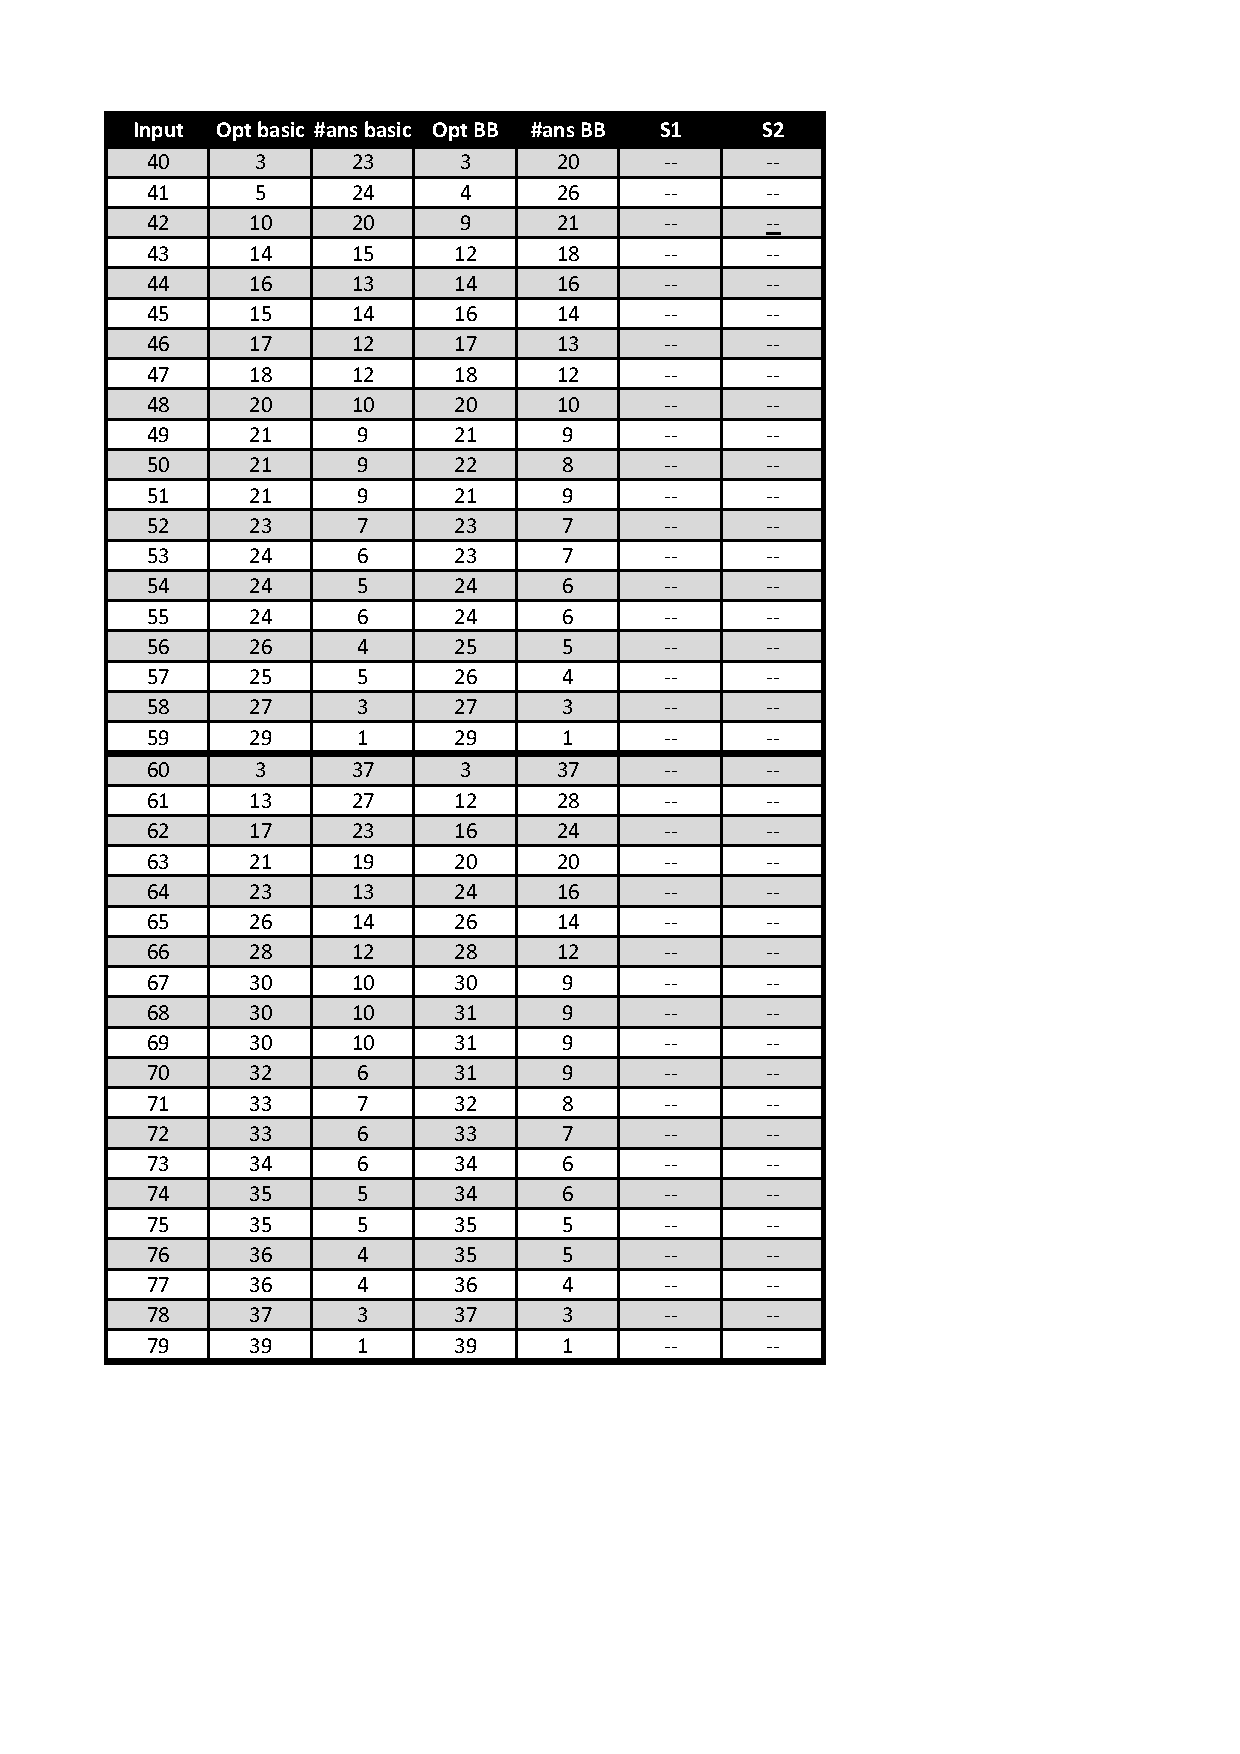
\includegraphics[width=350px]{Dati1.pdf}
	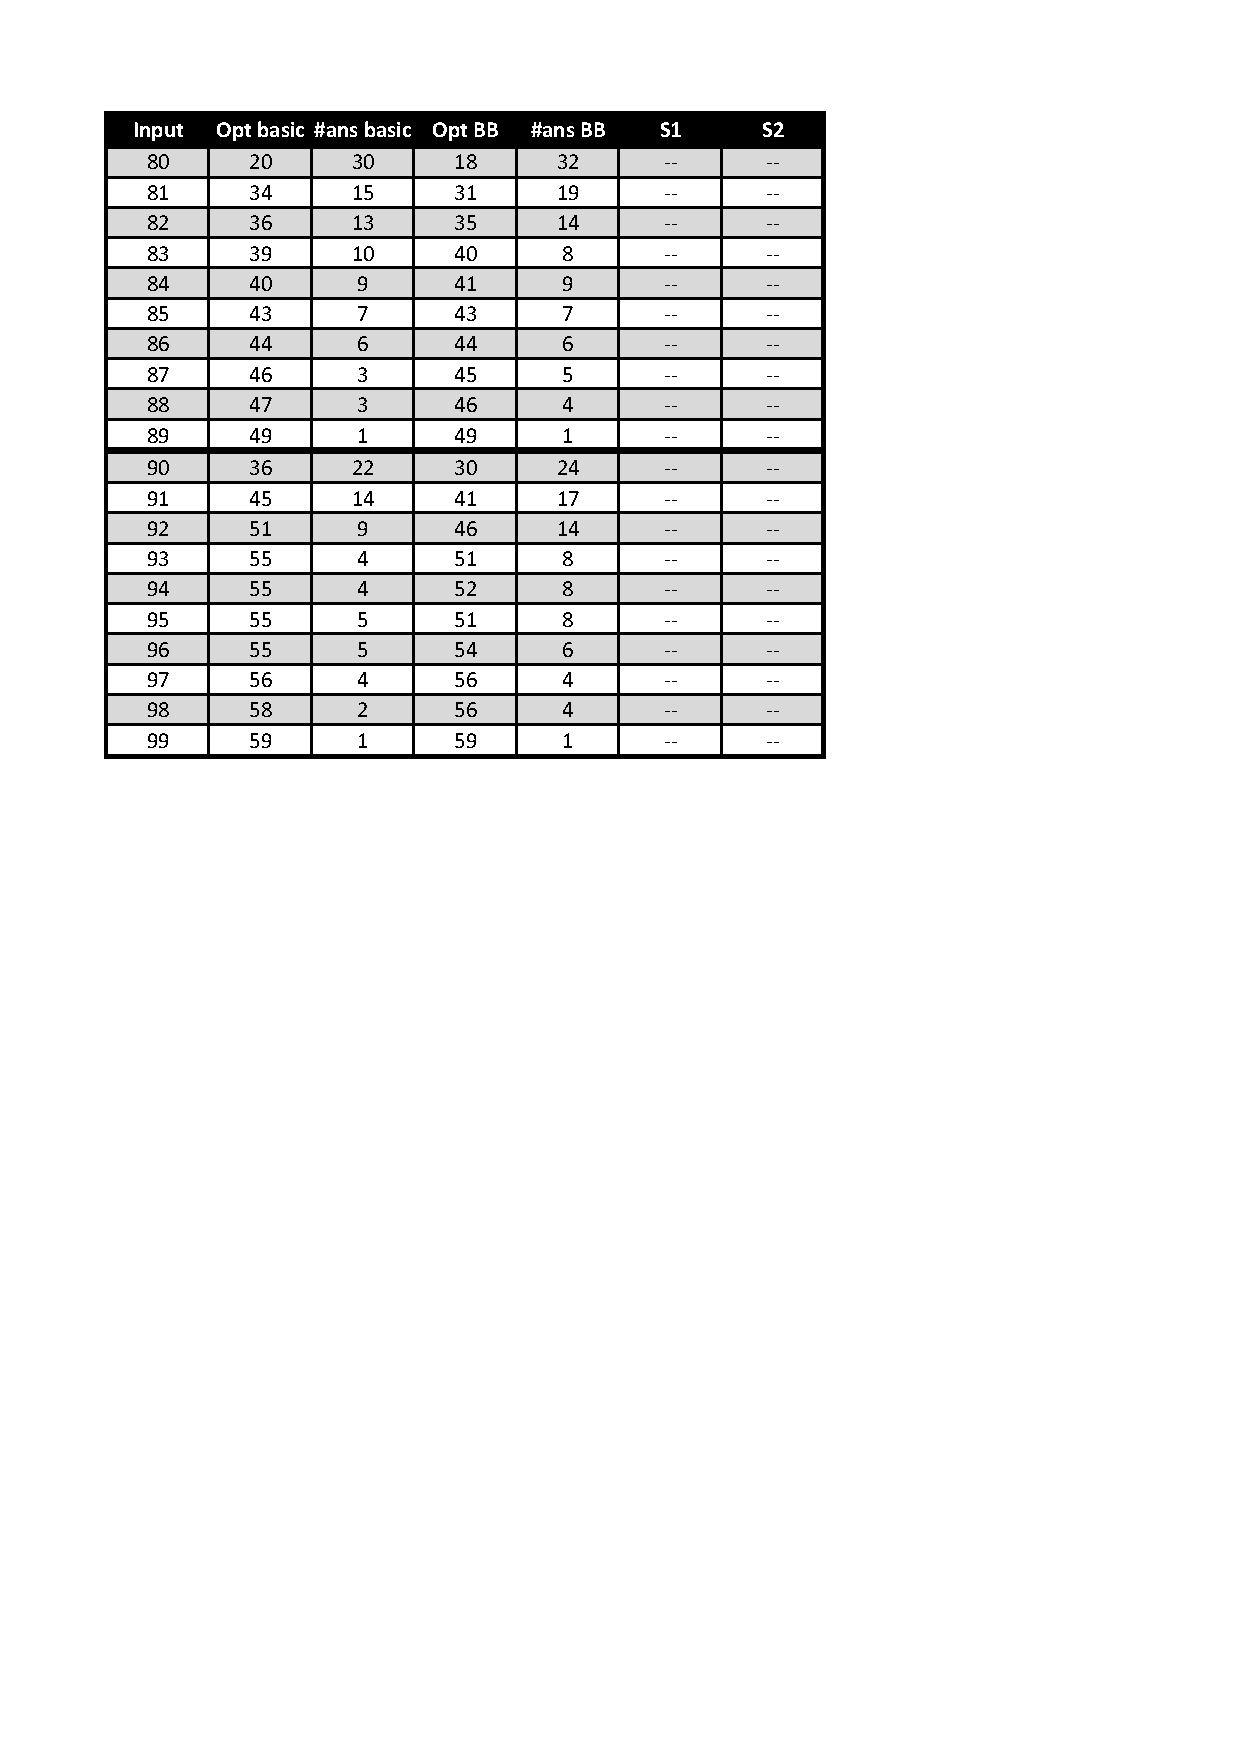
\includegraphics[width=350px]{Dati2.pdf}
%	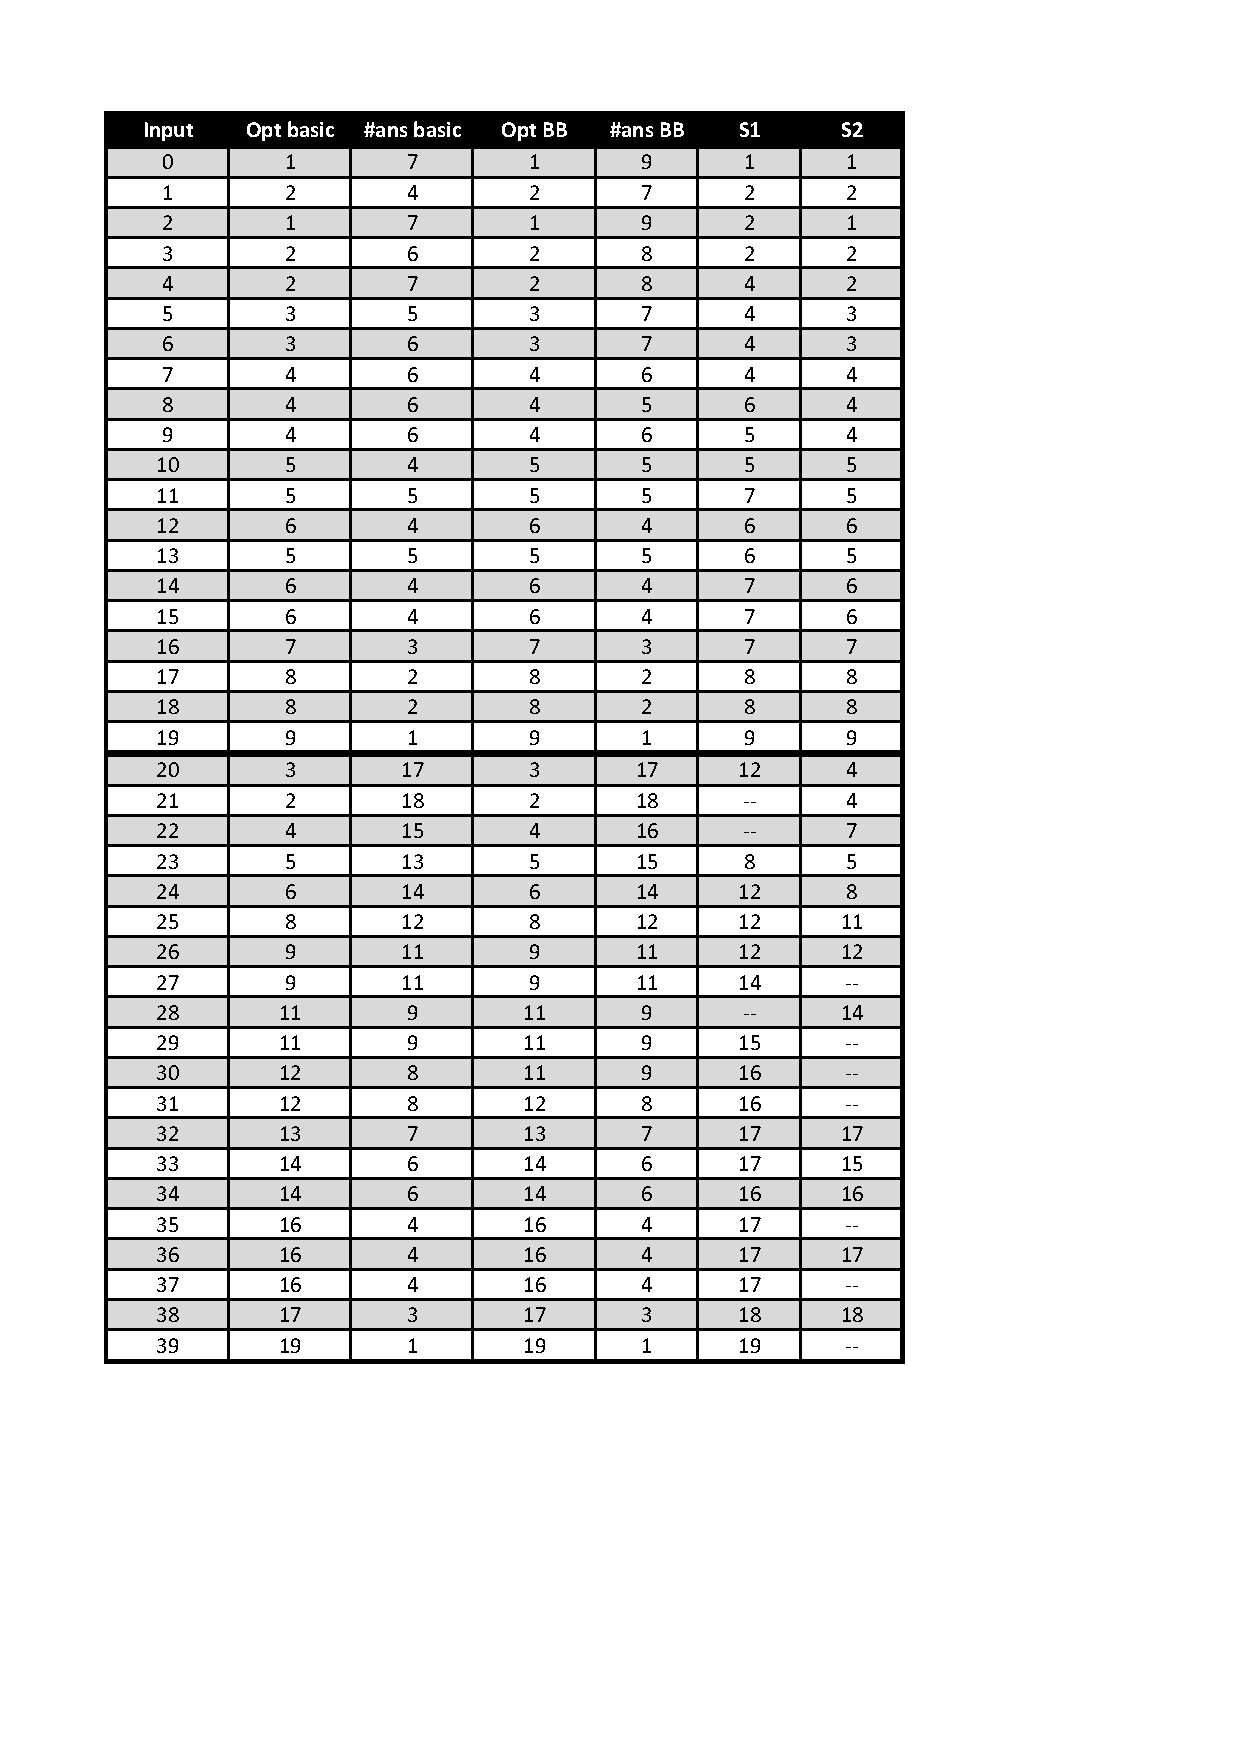
\includegraphics[width=350px]{Dati3.pdf}
\end{tabular}
\end{figure}


\end{document}